\documentclass[usenames,dvipsnames,10pt]{beamer} %\documentclass[usenames,dvipsnames,10pt,handout]{beamer}

\usepackage{pgfpages}
\usepackage{tabularx}
\usepackage{listings}

\mode<handout>{%
    \pgfpagesuselayout{4 on 1}[a4paper]
    \setbeameroption{show notes}
}

\usepackage{hutton/hutton}

\title{NetLogo CBR Extension}
\author{Doug Salt}
\institute{The James Hutton Institute}

\begin{document}

\begin{frame}[plain]
    \maketitle
\end{frame}

\begin{frame}{Structure}
    \begin{itemize}
        \item Basic concepts
        \item Core commands
        \item Other commands
        \item Simple example
        \item Example with bespoke lambda
    \end{itemize}
\end{frame}

\begin{frame}{Basic concepts}
    
    Normally a  case base consists of a series of cases, each of these cases
    consist of:

    \begin{itemize}
        \item state
        \item decision/activity
        \item outcome
    \end{itemize}

    The state can be anything such as the bank balance of the agent. The
    decision/activity might be to install central heating. The outcome might be
    straight forwardly yes or no. It might be probability, or it might some
    arbitrary decision/activity metric for use elsewhere.

\end{frame}

\begin{frame}{Basic concepts (continued)}

    A state and decision/activity are presented to the case base. The case base
    is searched for the closest match (if there is one) and the outcome of that
    match is given.

    \vspace{0.25cm}
    A NetLogo case consists of a state in any of the standard Netlogo
    variables, such as list, number, string, etc. This is strictly defined by
    the {\color{blue}\texttt{cbr:lambda}} which is the comparator program used
    to determine the "distance" the three cases:

    \begin{itemize}
		\item case A
		\item case B
		\item referent case R
    \end{itemize}

are relative to ecah other.

\end{frame}

\begin{frame}{Basic concepts (continued)}

    That is, if: 

    \begin{itemize}
        \item the case A is 'closer' to the referent case R than the case B
            using {\color{blue}\texttt{cbr:lamda}}  to the referent case R then
            {\color{blue}\texttt{cbr:lt}} is returned
        \item the case B is 'closer' to the referent case R than the case A
            using {\color{blue}\texttt{cbr:lamda}}  to the referent case R then
            {\color{blue}\texttt{cbr:gt}} is returned
        \item the case B is 'same distance' to the referent case R than the
            case A using {\color{blue}\texttt{cbr:lamda}}  to the referent case
            R then {\color{blue}\texttt{cbr:eq}} is returned
        \item the case B is 'closer' using {\color{blue}\texttt{cbr:lamda}}  to
            the referent case R then {\color{blue}\texttt{cbr:lt}} is returned
    \end{itemize}

\end{frame}

\begin{frame}{Basic concepts (continued)}

    Now when we need to decide whether a case matches one in the case base, we
    just bubble through the entire case base until we get the closest match or
    matches. The comparison method is always the same, i.e. the comparator
    program, denoted {\color{blue}\texttt{lamda}} herein, iff this routine when
    presented with three cases, can tell you which is closest to the referent
    case or whether they are comparable at all.

    \vspace{0.25cm}
    A default comparator program is provided, but this operates purely on state
    , does not consider the decision or outcome. For more information then
    please consult the NetLogo CBR documentation which may be found here.

    \vspace{0.25cm}
    \url{https://gitlab.com/doug.salt/cbr}


\end{frame}

\begin{frame}{Basic concepts (continued)}[fragile]

    The lamba can be specified in the code and must have the following
    parameters:

    \begin{itemize}
        \item case-base
        \item yes-case
        \item no-case
        \item reference-case
    \end{itemize}

    So the code for a bespoke comparator might look like this in NetLogo: 

    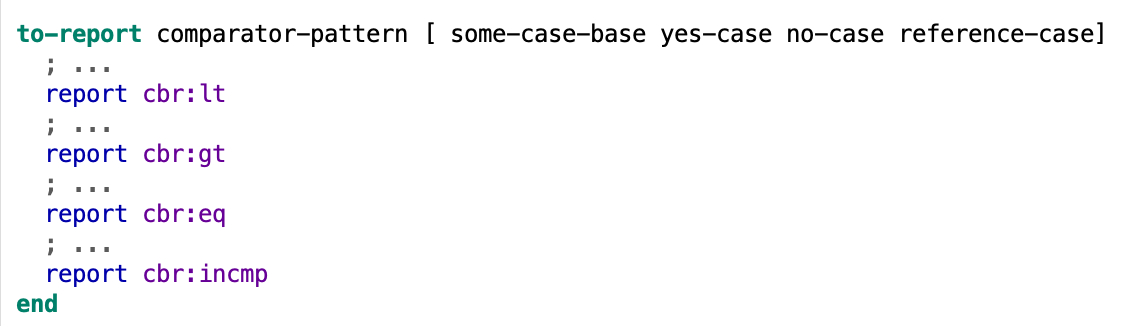
\includegraphics[width=9.5cm]{blank-comparator.png}

\end{frame}

\begin{frame}{Core commands}

    \begin{itemize}
        \item {\color{red}\texttt{cbr:new}} - creates a new case base.
        \item {\color{red}\texttt{cbr:add}} - adds a case to a case base
        \item {\color{red}\texttt{cbr:match}} - returns the closes match
        \item {\color{red}\texttt{cbr:outcome}} - queries a case for its outcome
        \item {\color{red}\texttt{cbr:decision}} - queries a case for its decision
        \item {\color{red}\texttt{cbr:lambda}} - set the default compartor progam
    \end{itemize}

\end{frame}

\begin{frame}{Other commands}

    \begin{itemize}
        \item {\color{green}\texttt{cbr:combine}} - combines two case bases.
        \item {\color{green}\texttt{cbr:all}} - returns all the cases as a list.
        \item {\color{green}\texttt{cbr:matches}} - returns more than one match if it exists.
        \item {\color{green}\texttt{cbr:state}} - gets the state of a particular case.
        \item {\color{green}\texttt{cbr:remove}} - removes a particular case.
        \item {\color{green}\texttt{cbr:set-time}} - sets the time at which a
            particular case base was created. This is done automatically at
            insertion into the case base. This commands just allows a degree of
            additional flexibility.
    \end{itemize}
\end{frame}

\begin{frame}{Other commands (continued)}

    \begin{itemize}
        \item {\color{green}\texttt{cbr:get-time}} - queries the querying of the
            time for a particular case.
        \item {\color{green}\texttt{cbr:set-earliest}} - sets the tick before
            which all case bases will be "forgotten".
        \item {\color{green}\texttt{cbr:get-earliest}} - allows the querying of
            the former.
        \item {\color{green}\texttt{cbr:forget}} - "forgets" all cases which are too old.
        \item {\color{green}\texttt{cbr:set-rank}} - sets the rank in the event of a tie breaker.
            the former.
        \item {\color{green}\texttt{cbr:get-rank}} - allows the querying of
            the former.
    \end{itemize}

\end{frame}

\begin{frame}{Easy example}

    {\color{blue}\texttt{cbr:new}} to set a new case base, so:

    \vspace{0.5cm}

    \small
    \texttt{set simple-case-base {\color{blue}cbr:new}}

    \vspace{0.5cm}

    \normalsize
    To add a new case then:

    \vspace{0.5cm}

    \small
    \texttt{set some-case {\color{blue}cbr:add}  simple-case-base [{\color{red}"lays eggs" "breathes air"}] {\color{red}"bird"} .01}

    \vspace{0.5cm}

    \normalsize
    where the first field is the case base object, the second is the state \texttt{[{\color{red}"lays eggs" "breathes air"} ]}; the third is the decision, \texttt{{\\color{red}}bird}, and the last is the outcome, which in this case is a probability of 0.1.

\end{frame}

\begin{frame}{Easy example (continued) }

    Add repeated multiple cases and then query using \texttt{{\color{blue}cbr:match}} or  \texttt{{\color{blue}cbr:matches}}, thus:

    \vspace{0.5cm}
    \small

    \texttt{let some-creature [ {\color{red}"lays eggs" "breathes air"} ]}

    \texttt{let result {\color{blue}cbr:match} simple-case-base some-creature {\color{red}"bird"}}

    \vspace{0.5cm}

    \normalsize
    So this constructs a "reference" case base to match, consisting of the state\texttt{some-creature}, and the decision \texttt{\color{red}"bird"}.

    \vspace{0.25cm}
    This is using the standard, in-build comparator. For more details on this please see the docmentation in the github repository \url{https://gitlab.com/doug.salt/cbr}.

\end{frame}
\begin{frame}{Easy example (continued) }

    So this here we another exmaple the code looks like eventually:

    \includegraphics[width=9.5cm]{"simple-example-code.png"}

\end{frame}

\begin{frame}{Easy example (continued) }

    And this is the result of clicking the "simple example" button.

    \includegraphics[width=9.5cm]{"simple-example-result.png"}

\end{frame}

\begin{frame}{Bespoke lambda}

    So the default comparator is not that brilliant, so we can implement our
    own:
    \vspace{0.5cm}

    \small
    \texttt{{\color{blue}cbr:lambda} simple-case-base some-comparator}

    \vspace{0.5cm}

    \normalsize

    Where the comparator starts with:

    \small
    \texttt{to-report [a-case-base src-case obj-case ref-case]}

    \vspace{0.5cm}

    \normalsize

    Where this routine must return \texttt{\color{blue}cbr:lt},
    \texttt{\color{blue}cbr:gt}, \texttt{\color{blue}cbr:eq} or
    \texttt{\color{blue}cbr:incmp}.  And that is it.

    \vspace{0.5cm}

    The only small problem being that there is a bug in the comparator by the
    looks of things which needs fixing.


\end{frame}

\begin{frame}

    \vspace{1cm}

    Any questions?

    \vspace{1cm}

    Thank you very much
\finalpage
\end{frame}

\end{document}

